%% Example data sheet
%% Feel free to modify and use this file for any purpose, under
%% either the LaTeX Project Public License or under public domain.

% Options here are passed to the article class.
% Most common options: 10pt, 11pt, 12pt
\documentclass[10pt]{datasheet}

% Input encoding and typographical rules for English language
\usepackage[utf8]{inputenc}
\usepackage[english]{babel}
\usepackage[english]{isodate}

\usepackage{setspace}
% tikz is used to draw images in this example, but you can
% also use \includegraphics{}.
\usepackage{tikz}
\usepackage{pgfplots}
\usepackage{circuitikz}
\usetikzlibrary{calc}

\usepackage{enumitem}

\usepackage[T1]{fontenc}
\usepackage{libertine}%% Only as example for the romans/sans fonts
\usepackage[scaled=0.85]{beramono}


\setlength{\parskip}{0.7em} 

\usepackage{titlesec}
\titlespacing*{\section}
{0pt}{0pt}{0pt}

\usepackage{graphicx}
\graphicspath{ {.} }
\setlength{\tabcolsep}{4pt}

%\setstretch {0.75}

\newcommand*\circled[1]{\tikz[baseline=(char.base)]{
		\node[shape=circle,draw,inner sep=2pt, fill=white] (char) {#1};}}


% These define global texts that are used in headers and titles.
\title{
\includegraphics[height=2cm]{logo} \raisebox{1\height}{Hardware mini-badge "P2N"}}
\author{End Summer Camp}
\date{Settembre 2024}
\company{https://t.me/endsummercamp}
\author{Kezi, ESC Badge Team}
\companylogo{
\includegraphics[scale=0.6]{logo}}

\begin{document}
	\maketitle
	
	\section{Introduzione}
	Hai fra le mani il badge "P2N", ovvero il gadget Open Source dell'evento End Summer Camp 2024.
	Rispetto alla versione "P1N", questo dispositivo è basato sul chip RP2040, introduce una splendida matrice LED 3x3 ARGB, molteplici interfacce,
	il 110\% di effetti luminosi in più ed un ricevitore infrarossi.
	
	\section{Avvertenze}
	Il dispositivo può emettere forti e improvvise irradiazioni fotoniche.
	Prima dell'accensione, indossare gli appositi occhiali da saldatura
	(non inclusi).
	
	\section{Funzionalità}
	\begin{tabular}{l l}
		  \begin{minipage}{1.45in}

				\begin{enumerate}[itemsep=1pt]
				\item{GPIO di espansione}
				\item{LED di stato}
				\item{JTAG (Tag-Connect)}
				\item{RP2040}
				\item{USB power+dati}
				\item{LED/trasmettitore IR}

			\end{enumerate} 
			
			\end{minipage}&
				  \begin{minipage}{2in}

			\begin{enumerate}[itemsep=1pt]
			\setcounter{enumi}{6}
			\item{pulsante USER}
			\item{pulsante BOOT}
			\item{pad alimentazione}
			\item{espansione stringa LED}
			\item{ricevitore infrarossi}
			\item LED ws2812b/sk6812
			\end{enumerate} 
			
		\end{minipage}
	\end{tabular}

	
	\section{Utilizzo}
	
	\begin{itemize}[itemsep=1pt]
		\item{collegare l'USB C ad un'alimentazione a 5V}
		\item{per variare le 12+ animazioni, premere USER}
		\item{per regolare le 4 intensità, tenere premuto USER}
		\item{per attivare la torcia, tenere premuto USER all'avvio}
		\item{per il bootloader USB, tenere premuto BOOT all'avvio}
	\end{itemize}
	

	\begin{center}

		\begin{tikzpicture}
	\draw (0, 0) node[inner sep=0] {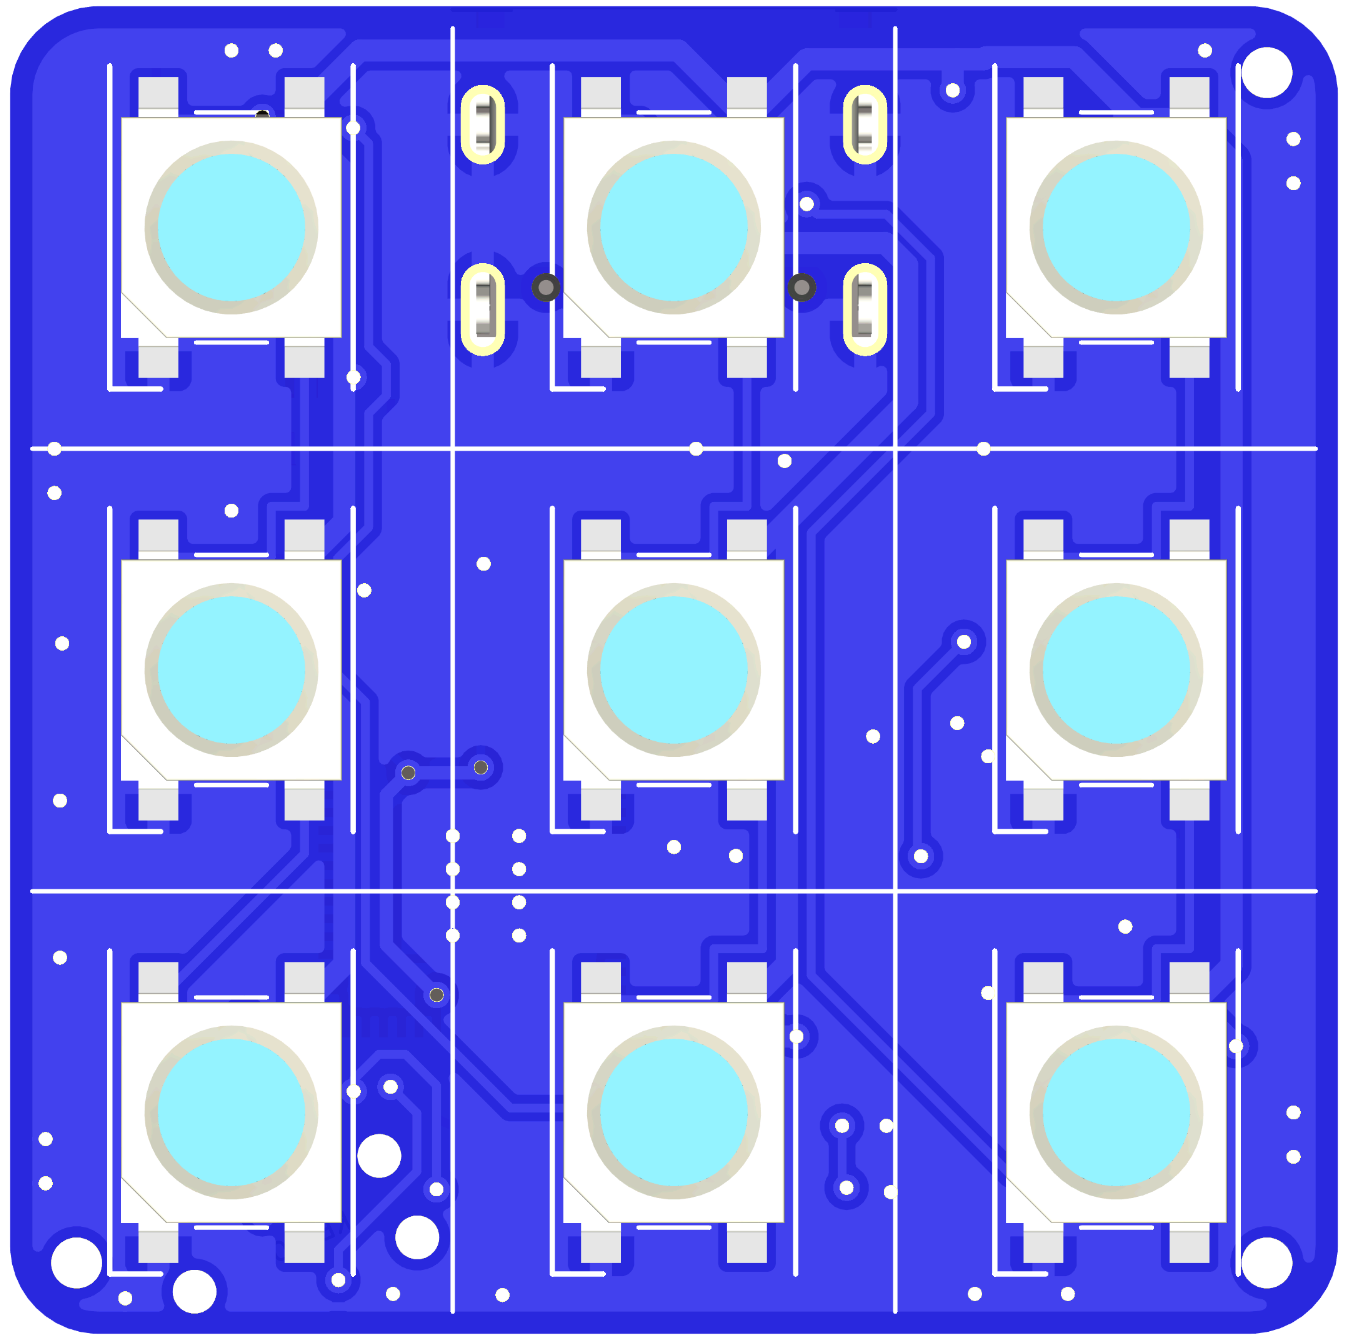
\includegraphics[width=3cm]{back}};
	\draw (1, 1) node {\circled{12}};

\end{tikzpicture}
	\end{center}
		Visione frontale, con la porta USB rivolta in alto. 
		
		\section{Ricevitore Infrarossi}
		Puoi controllare il badge a distanza attraverso infrarossi NEC (o variante Samsung) come da info allegate al repository.
	
	% Switch to next column
	\vfill\break
	\vspace*{-30pt}
	\begin{center}
		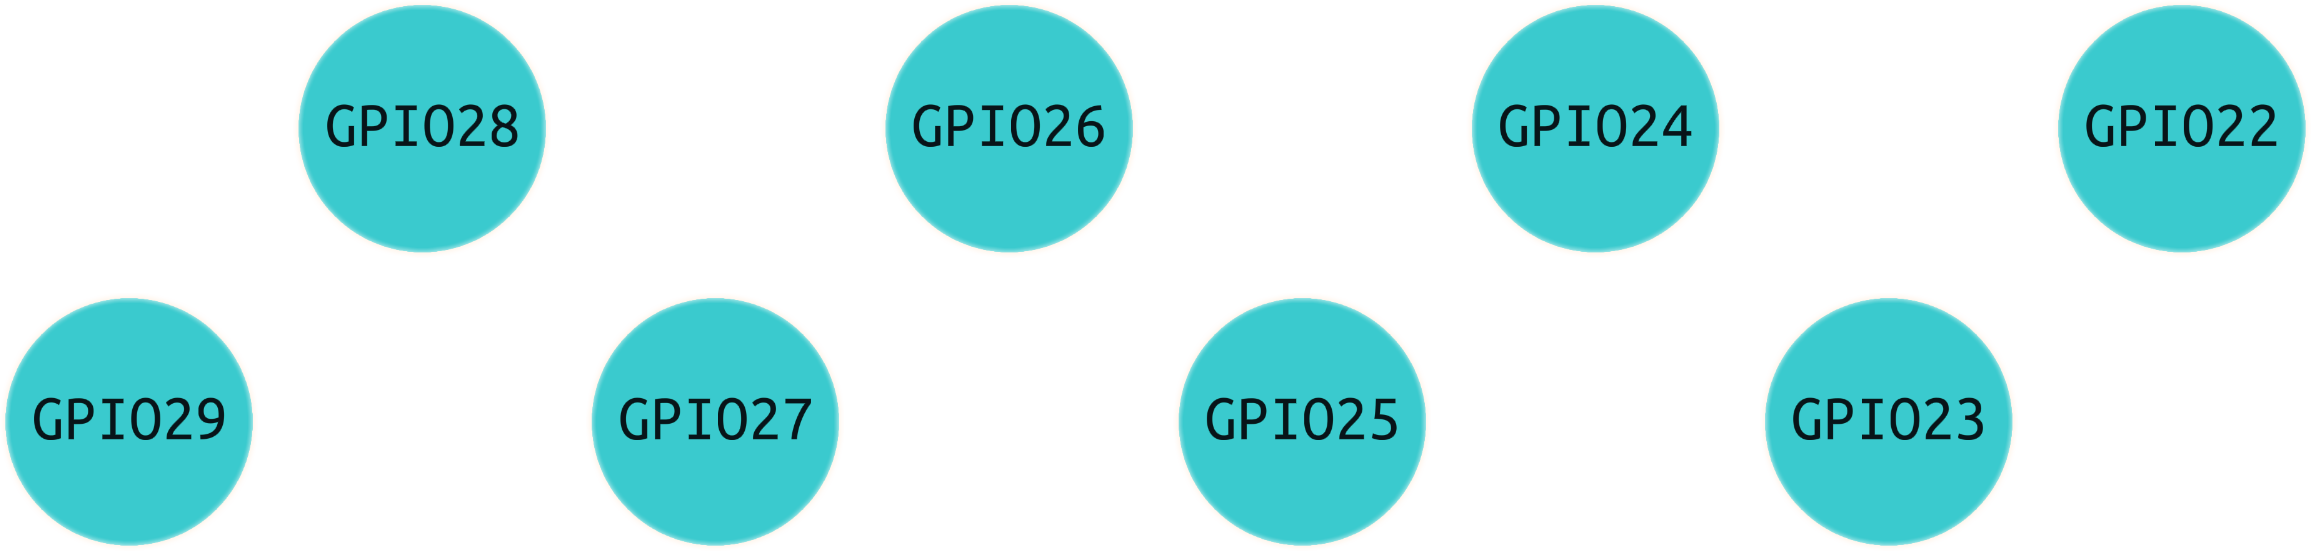
\includegraphics[scale=0.75]{gpio}

		\begin{tikzpicture}
			\draw (0, 0) node[inner sep=0] {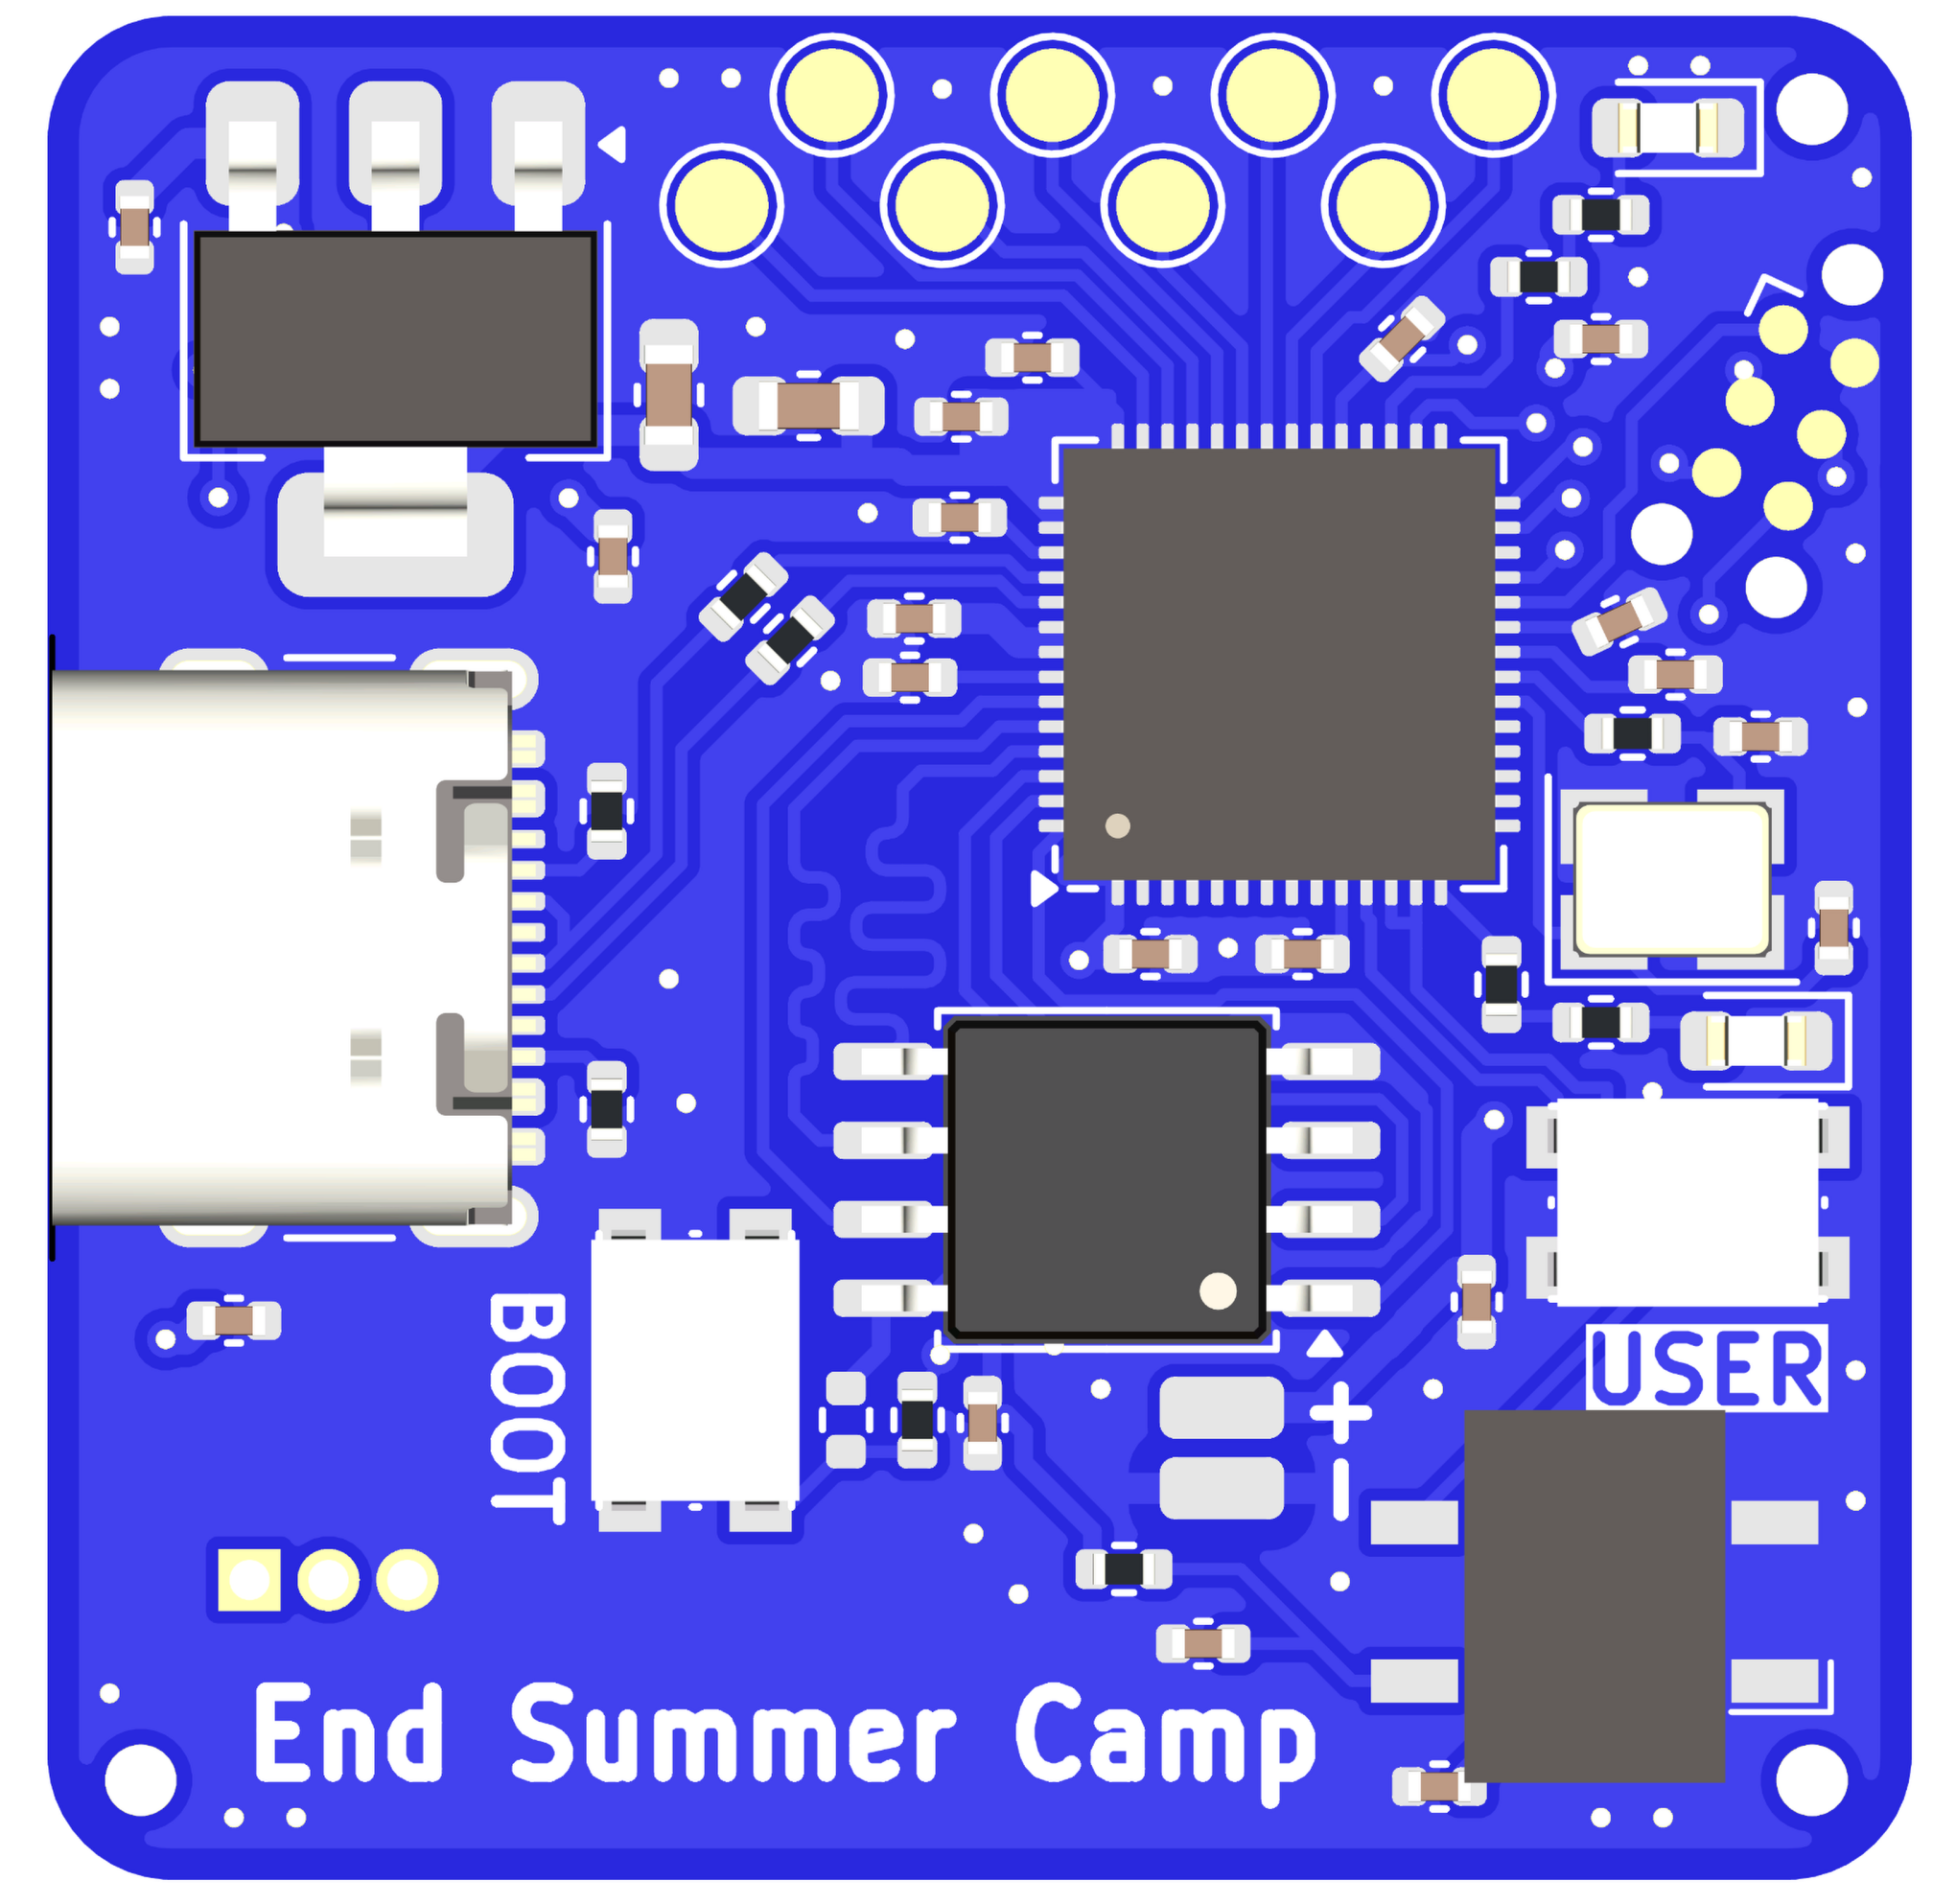
\includegraphics[width=6.4cm]{front}};
			\draw (0, 2.8) node {\circled{1}};
			\draw (2.8, 2.8) node {\circled{2}};
			\draw (2.8, 1.8) node {\circled{3}};
			\draw (1, 1) node {\circled{4}};
			\draw (-2, 0) node {\circled{5}};
			\draw (3.1, -0.3) node {\circled{6}};
			\draw (2.45, -0.81) node {\circled{7}};
			\draw (-0.9, -1.4) node {\circled{8}};
			\draw (0.7, -1.65) node {\circled{9}};
			\draw (-2.15, -1.8) node {\circled{10}};
			\draw (2.1, -2.2) node {\circled{11}};
		\end{tikzpicture}
		
	\end{center}
\vspace*{-10pt}
\section{Porta USB}
Collegando il badge ad una porta USB di un computer, si aggiungeranno 4 interfacce. Ad esempio:
\vspace*{-10pt}
\begin{itemize}[itemsep=1pt]
	\item {\textbf{\texttt{/dev/midi1}}, si possono regolare i colori di ogni LED inviando eventi MIDI al badge: ogni canale (RGB) di ogni LED è una "nota", mentre l'intensità è il valore MIDI (da 0-127 mappato a 0-255)}
	\item{\textbf{\texttt{/dev/ttyACM0}}, seriale di controllo, utilizzabile con il tool da linea di comando ufficiale, o con qualsiasi altro tool che implementa il protocollo secondo lo schema \textit{Cap'n Proto} presente nel sorgente}
	\item{\textbf{\texttt{/dev/ttyACM1}}, seriale di debug che trasmette log}
	\item{\textbf{\texttt{/dev/input/event0}}}, il badge si presenta come tastiera HID ricevendo i tasti di un telecomando IR supportato
\end{itemize}
\vspace*{-10pt}
\section{Interfaccia a Riga di Comando}
È disponibile un tool per controllare il badge da un computer attraverso la sua porta USB, per
controllare i LED e il transceiver infrarosso.
\vspace*{-5pt}
\section{Sorgente e altra Documentazione}
Tutto il materiale è organizzato in un unico repository, contenente hardware, firmware e tool da linea di comando.\\
\texttt{https://github.com/endsummercamp/minibadge}
%\section{Note}
%Il badge \textbf{non} contiene un BMS, consultare lo schema prima di collegare una batteria ai pad di alimentazione.
	
\end{document}


